\chapter{Experimental Setup}
\label{ch:ExperimentalSetup}

\section{Sensors}
\subsection{\glsentrytext{imu}}
\missingfigure{Picture of myAHRS+ or/and ZED2i}
Two different \gls{imu}s will be used for the experiment.
The first one being the WITHROBOT myAHRS+, a low cost high performance \gls{ahrs}.
An \gls{ahrs} contains an \gls{imu} and outputs the raw data but also has an integrated Kalman filter which calculates the pose in form of quaternion or euler angles.
The second \gls{imu} used during the experiment is integrated in the ZED 2i Stereo camera.
The specifications of each \gls{imu} can be read in table
\begin{table}[ht]
	\centering
	\caption{Comparison of the two used \gls{imu}s}
	\label{tab:imu_datasheets}
	\begin{tabular}[t]{lcc}
		\toprule
		                            & \textbf{myAHRS+}                                       & \textbf{ZED 2i \gls{imu}}                              \\
		\midrule
		Accelerometer range         & $\pm\SI{16}{\g}$                                       & $\pm\SI{8}{\g}$                                        \\
		Gyroscope range             & $\pm\SI{2000}{\degree\per\second}$                     & $\pm\SI{1000}{\degree\per\second}$                     \\
		Magnetometer range          & $\pm\SI{1200}{\micro\tesla}$                           & $\pm\SI{2500}{\micro\tesla}$                           \\
		Rate                        & \SI{100}{\hertz}                                       & \SI{400}{\hertz}                                       \\
		Accelerometer noise density & \SI{4.502e-3}{\metre\per\second(1\per\sqrt{\second})}  & \SI{1.148e-3}{\metre\per\second(1\per\sqrt{\second})}  \\
		Accelerometer random walk   & \SI{7.337e-5}{\metre\per\second\squared\sqrt{\second}} & \SI{6.458e-5}{\metre\per\second\squared\sqrt{\second}} \\
		Gyroscope noise density     & \SI{1.674e-4}{\radian\per\sqrt{\second}}               & \SI{8.254e-5}{\radian\per\sqrt{\second}}               \\
		Gyroscope random walk       & \SI{5.042e-6}{\radian\per\second\sqrt{\second}}        & \SI{1.632e-7}{\radian\per\second\sqrt{\second}}        \\
		\bottomrule
	\end{tabular}
\end{table}%
\itodo{Add cite to manuals}
\iimprov{Values and units of random walk and noise density probably wrong (measured them myself)}
It offers an micro-USB interface and runs with up to \SI{100}{\Hz}.
It can capture a change of $\pm$2000 dps (degrees per second), $\pm$16 $g$ and $\pm$\SI{1200}{\micro\tesla}.
During the experiment only a fraction of this range is expected to be reached, hence the sensor seems suitable.
Besides the hardware the unit already has an Extended Kalman Filter (EKF) on board.
The EKF fuses the measurements of the three sensors and estimates a quaternion (and sth else?) from it.
But this will not be used.
\iimprov{More about both \gls{imu}}


\subsection{\glsentrytext{lidar}}
Two different \gls{lidar}s will be used during the experiment.
The RS-Bpearl and the Velodyne UltraPuck.
The most relevant specifications of the two \gls{lidar}s can be seen in table \ref{tab:lidar_datasheets}.
Both are mechanical \gls{lidar}s and have the same number of laser channels, but the Velodyne has a significant better vertical resolution, due to the smaller vertical \gls{fov}.
\begin{table}[ht]
	\centering
	% todo: Manual citation prop wrong
	\caption{Comparison of the two used \acrshort{lidar}s \cite{RoboSense2020}\cite{Velodyne2018}}
	\label{tab:lidar_datasheets}
	\begin{tabular}[t]{lcc}
		\toprule
		                      & \textbf{RS-Bpearl}          & \textbf{Velodyne Ultra Puck}                  \\
		\midrule
		Channels              & 32                          & 32                                            \\
		Range                 & \SI{100}{\metre}            & \SI{200}{\metre}                              \\
		Range accuracy        & $\pm\SI{3}{\centi\metre}$   & $\pm\SI{3}{\centi\metre}$                     \\
		Horizontal \gls{fov}  & \SI{360}{\degree}           & \SI{360}{\degree}                             \\
		Vertical \gls{fov}    & \SI{90}{\degree}            & \SI{40}{\degree} (\SIrange{-25}{15}{\degree}) \\
		Horizontal resolution & \SIrange{0.2}{0.4}{\degree} & \SIrange{0.1}{0.4}{\degree}                   \\
		Vertical resolution   & \SI{2.81}{\degree}          & \SI{0.33}{\degree}                            \\
		Frame rate            & \SIrange{10}{20}{\hertz}    & \SIrange{5}{20}{\hertz}                       \\
		Laser wavelength      & \SI{905}{\nano\metre}       & \SI{903}{\nano\metre}                         \\
		% \midrule
		Points per second     & 576,000                     & 600,000                                       \\
		\bottomrule
	\end{tabular}
\end{table}%
\begin{figure}[htb]
	\centering
	\begin{subfigure}{0.3\textwidth}
		\centering
		\includegraphics[width=\textwidth]{Robosense.png}
		\caption{Robosense RS-Bpearl \cite{RoboSense2020}}
		\label{fig:lidar_robosense}
	\end{subfigure}
	% \hfill
	\begin{subfigure}{0.3\textwidth}
		\centering
		\includegraphics[width=\textwidth]{Velodyne.png}
		\caption{Velodyne Ultra puck \cite{Velodyne2018}}
		\label{fig:lidar_velodyne}
	\end{subfigure}
	\caption{The two used \gls{lidar}s}
	\label{fig:lidars_used}
\end{figure}



\section{Sensor placement}
The \gls{imu} must be placed on a rigid point of the car, such that the \gls{imu}'s position stays always the same relative to the car.
Other then that it should also be placed in the transversal center? to guarantee that the centripetal acceleration is not skewed towards one side.
The \gls{imu} was placed on the roof center.
\begin{figure}[htpb]
	\centering
	\documentclass{standalone}
\usepackage{tikz}
\usepackage{tikz-dimline}		% Dimension (measure) lines for TikZ
\usetikzlibrary{angles, calc, decorations.pathmorphing, quotes, spy}

\begin{document}
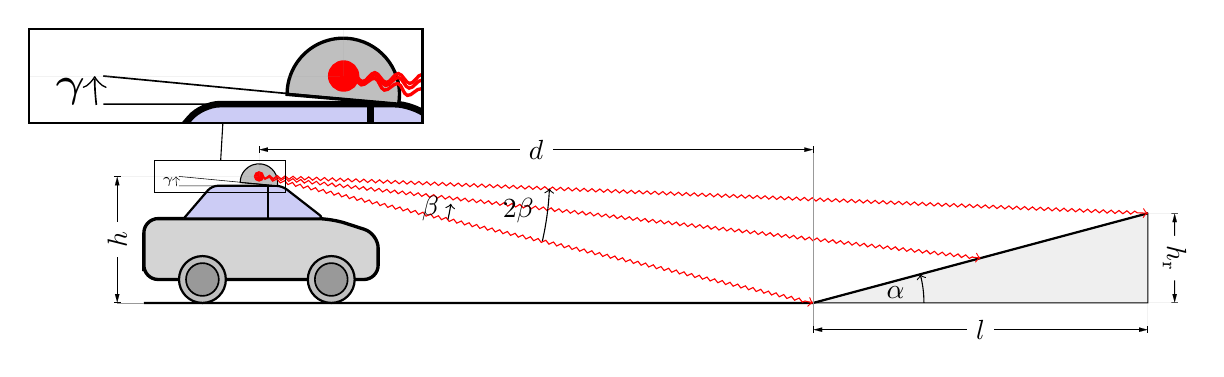
\begin{tikzpicture}[scale=0.85, spy using outlines={black, rectangle, magnification=3, width=5cm, height=1.2cm, connect spies}]
    % Define/Calc ramp parameters
    % Ramp length
    \def\rl{5};
    % Ramp angle [deg]
    \def\ra{15};
    % Ramp height
    \def\rh{{tan(\ra)*\rl}};
    % Distance of measurement line
    \def\dd{.4cm}

    % RAMP
    % Define the points
    \coordinate (A) at (0,0);
    \coordinate (B) at ($(A) + (\rl,0)$);
    \coordinate (C) at ($(B) + (0,\rh)$);
    % Draw and fill ramp
    \filldraw[draw=black, fill=lightgray!25] (A) -- (B) -- (C) -- cycle;
    % Draw angle
    \path (A) -- (B)
    pic[draw, ->, angle radius=40pt,
    angle eccentricity=0.75, "$\alpha$"]{angle=B--A--C};
    % Ground and helpers
    \coordinate (D) at ($(A) + (-10,0)$);
    \draw [thick] (D) -- (A) -- (C);

    % CAR
    \begin{scope}[scale=0.7]
        % Car height
        \def\ch{2}
        % Car length
        \def\cl{5}
        % Car body height
        \def\bh{\ch*0.65}
        % Roof length
        \def\rl{\cl*0.6}
        % Roof height
        \def\rh{\ch*0.35}
        % Car tilt angle
        \def\ct{6}
        % Anchor point is southwest
        \coordinate (b) at ($(D) + (0,0.5)$);
        % Offset to roof and wheels
        \coordinate (r) at ($(b) +(\cl*0.17,\ch*0.65)$);
        \coordinate (w) at ($(b) + (\cl*0.25,0)$);

        % Body
        \draw[black, fill=black!17, rounded corners=1.2ex, very thick]
        (b) -- ++(0,\bh) -- ++(\cl*1/5,0) --  ++(\cl*3/5,0) -- ++(\cl*1/5,-\bh*0.25)
        -- ++(0, -\bh*0.75) -- (b) -- cycle;
        % Roof
        \draw[very thick, rounded corners=0.5ex, fill=black!20!blue!20!white,thick]
        (r) -- ++(0.2*\rl,\rh) -- ++(0.5*\rl,0) -- ++(0.3*\rl,-\rh) -- (r);
        % \draw[thick] ($(r) + (\cl*0.5,\bh)$) -- ++(0,\rh);
        \draw[thick] (r)++(\rl*0.6,0) -- ++(0,\rh);

        % Wheels
        \draw[draw=black,fill=gray!50,thick] (w) circle (.5);
        \draw[draw=black,fill=gray!50,thick] (w) ++(\cl*0.55,0) circle (.5);
        % Inner wheels
        \draw[draw=black,fill=gray!80,semithick] (w) circle (.35);
        \draw[draw=black,fill=gray!80,semithick] (w) ++(\cl*0.55,0) circle (.35);

        % Lidar
        \draw[black, fill=gray!50] ($(r) + (\cl*0.40,\rh)$) coordinate (le) arc(-10:180:0.4) --cycle;

        % Car middle point
        \coordinate (m) at (\cl*0.5, \bh*0.5);
        % Lidar middle point
        \coordinate (lm) at ($(le) + (-0.39,0.2)$);
        \filldraw[red] (lm) circle(.1);
        % lidar mount angle
        % \draw (lm) -- ($(lm) + (-3, 0)$);
        % \path (A) -- (B)
        \coordinate (blob) at ($(le) + (-2.1, 0)$);
        \coordinate (blub) at ($(le) + (-2.1, 0.2)$);
        % \draw (blob) circle (.1);
        % \draw (blub) circle (.1);
        \draw[draw=black, very thin] (blob) -- (le) -- (blub)
        pic[draw, <-, angle radius=30pt,
        angle eccentricity=1.1, "\tiny $\gamma$"]{angle=blub--lm--blob};

        % Laser lines
        \draw[->,color=red,decorate,decoration={snake,amplitude=.2mm,segment length=1mm,post length=1mm}] (lm) -- (A);
        \draw[->,color=red,decorate,decoration={snake,amplitude=.2mm,segment length=1mm,post length=1mm}] (lm) -- ($(A)!0.5!(C)$);
        \draw[->,color=red,decorate,decoration={snake,amplitude=.2mm,segment length=1mm,post length=1mm}] (lm) -- ($(A)!1!(C)$);
        \path (lm) -- (A)
        pic[draw, ->, angle radius=70pt, angle eccentricity=0.9,
        "$\beta$"]{angle=A--lm--B};
        \path (lm) -- (C)
        pic[draw, ->, angle radius=105pt, angle eccentricity=0.9,
        "$2\beta$"]{angle=A--lm--C};
    \end{scope}

    % \dimline[extension start length=-\dd, extension end length=-\dd] {($(D)+(0,-\dd)$)}{($(A)+(0,-\dd)$)}{$d$};
    % \dimline[extension start length=\dd, extension end length=\dd] {($(A)+(0,-\dd)$)}{($(A)!0.4!(D)+(0,-\dd)$)}{$d$};
    \dimline[extension start length=\dd, extension end length=\dd+1.9cm] {($(lm)+(0,\dd)$)}{($(lm -| A)+(0,\dd)$)}{$d$};
    \dimline[extension start length=-\dd, extension end length=-\dd] {($(A)+(0,-\dd)$)}{($(B)+(0,-\dd)$)}{$l$};
    \dimline[extension start length=-\dd, extension end length=-\dd] {($(B)+(\dd,0)$)}{($(C)+(\dd,0)$)}{$h_\mathrm{r}$};
    \dimline[extension start length=\dd, extension end length=\dd+1.7cm] {($(D)+(-\dd,0)$)}{($(lm -| D)+(-\dd,0)$)}{$h$};
    % \draw (D) -- (lm -| D);
    % \dimline[extension start length=-\dd, extension end length=-\dd] {($(lm)+(\dd,0)$)}{($(C)+(\dd,0)$)}{$h_2$};
    % \dimline[extension start length=\dd, extension end length=\dd] {($(A)+(0,\dd)$)}{($(C)+(0,\dd)$)}{$d$};
    % \spy on ($(lm)!.05!(A)$) in node at (3,4);

    % \spy[black] on ($(lm) + (-0.42, 0)$) in node at (3,4);
    \spy on ($(lm) + (-0.5, 0)$) in node at ($(lm) + (-0.5, 1.5)$);

\end{tikzpicture}
\end{document}
	\caption{Mounting of the \acrshort{lidar}}
	\label{fig:tikz_lidar_mount}
\end{figure}
\begin{table}[htbp]
	\centering
	\caption{Some params}
	\label{tab:vals}
	\begin{tabular}[t]{clc}
		\toprule
		\textbf{Variable} & \textbf{Description}                                   & \textbf{Unit} \\
		\midrule
		$h_\mathrm{l} $   & \gls{lidar} height above ground                        & \si{\metre}   \\
		$d$               & Distance to ramp                                       & \si{\metre}   \\
		$h_\mathrm{r}$    & Height of ramp                                         & \si{\metre}   \\
		$l_\mathrm{w}$    & Light travel distance from ramp start to contact point & \si{\metre}   \\
		$d_\mathrm{w}$    & Distance from ramp start to contact point              & \si{\metre}   \\
		$\alpha$          & Ramp angle                                             & \si{\degree}  \\
		$\beta$           & \gls{lidar} mount angle                                & \si{\degree}  \\
		$\gamma$          & Tue angle?!                                            & \si{\degree}  \\
		$\epsilon$        & \gls{lidar} vertical resolution                        & \si{\degree}  \\
		$n$               & Number of laser channels                               &               \\
		\bottomrule
	\end{tabular}
\end{table}

The \gls{lidar} will be placed on top of the car, to get a greater \gls{fov}.
The pitch angle $\beta$ at which the \gls{lidar} will be mounted should be chosen such that the number of points in the area at the beginning of the ramp are maximized.
This allows for the most accurate distinction between planes of different inclination angles and therefore also a good distance estimation.
Because the distance to the ramp is not constant due to the movement of the car, the optimization can only be done for a specific distance.
The coordinates at which the lasers hit the ground and ramp depend on the height of the \gls{lidar} $h_\mathrm{l}$, the distance to the ramp $d$, the angle of the ramp $\alpha$, the angle $\beta$ at which the \gls{lidar} has been mounted on the car and finally on the vertical resolution and \gls{fov} of the \gls{lidar}.
The coordinates can be calculated in the following way.\\
The angle $\gamma$ between the NOT ground and each laser wave is defined as
\begin{equation}
	\gamma = \beta - i\epsilon
\end{equation}
with $i \in \mathbb{N}, 0\dots n$ being the "laserID" starting from the lowest opening angle and going to the highest.
On flat ground the distance at which the laser waves hit the ground can be calculated with
\begin{equation}
	x = \tan(\ang{90} - \gamma) h_\mathrm{l}.
	\label{eq:ground_points}
\end{equation}
With a ramp, the assumption from \ref{eq:ground_points} does not hold anymore.
The light does not travel as far.
The height above ground, when the light is at the beginning of the ramp can be calculated with
\begin{equation}
	h_\mathrm{w,start} = h_\mathrm{l} - d\tan(\gamma)
\end{equation}
The distance $l_\mathrm{w}$ which the light travels from the beginning of the ramp to the contact point with the ramp can be calculated using the law of sines
\begin{align}
	l_\mathrm{w} & = \frac{h_\mathrm{w,start} }{\sin(\alpha + \gamma)} \sin(\ang{90} - \alpha) \\
	             & = \frac{h_\mathrm{w,start} }{\sin(\alpha + \gamma)} \cos(-\alpha)
\end{align}
The travelled distance along the x-axis from the start of the ramp to the contact point is then
\begin{equation}
	d_\mathrm{w}  = l_\mathrm{w} \sin(\ang{90} - 2\alpha - \gamma)
\end{equation}
which results in the total x distance from the \gls{lidar}
\begin{equation}
	d_\mathrm{hit} = d + d_\mathrm{w}.
\end{equation}
\iquest{Instead of "long" derivation, just use the final equation?}
\begin{equation}
	d_\mathrm{hit} = d + \frac{h_\mathrm{l} - d\tan(\gamma)}{\sin(\alpha + \gamma)} \cos(-\alpha) \sin(\ang{90} - 2\alpha - \gamma)
\end{equation}
Using the formulas the optimal mounting pitch angle $\beta$ for the two \gls{lidar}s has been found with $\beta_\mathrm{velodyne} = \ang{0}$ and $\beta_\mathrm{robos} = \ang{20}$.
\iimprov{Improve text and table param description}


\section{Car}
The car used in the experiment is an eGolf 2017.
The car has been "hacked" which allows for the reading of the wheel ticks.
Because the ... mode is used, the output power of the motor is limited and the maximum speed is capped at \SI{5}{\kilo\metre\per\hour}.
The traversing of ramps is not possible and this mode, which is why a the normal mode was used for the recording where the ramp was fully driven up.
But in the normal driving mode the wheel speed readings were not available.
The car has a pc in the booth, at which the sensors were connected to.
\iimprov{Text is bad}
\missingfigure{Picture of eGolf}
\todoin{\begin{itemize}
		\item Some stats as height, track width etc, electric car hence less vibrations
		\item Connection setup (maybe own section or maybe not interesting at all)
	\end{itemize}
}



\section{Garage}
\missingfigure{Picture of ramps and/or figure of ramps showing angles}
\itodo{Think of a good way to measure the true angle of the ramps}